\documentclass[10pt,xcolor=dvipsnames,compress]{beamer}

\usepackage{danny_theme}
\usepackage{danny_style}
\usepackage{hyperref}
%\usepackage[algoruled,longend]{algorithm2e}
\usepackage{array}
\usepackage{graphicx}
\usepackage{amsmath}
\newcolumntype{C}{>{\centering\arraybackslash} m{1.3in} }
\newcolumntype{M}{>{\centering\arraybackslash} m{1.in} }
\everymath{\displaystyle}
\long\def\/*#1*/{}

\beamertemplatenavigationsymbolsempty


%===============================================================================
% 					  Presentation Title and Author  
%===============================================================================
\title[Supercapacitor Inadequecy]{
Inadequecy Representation in Models of Supercapacitor Batteries}
\subtitle{Part II: updates on inadequacy formulation}

\author[Danial Faghihi]{Danial Faghihi}

\institute[ICES]{Institute for Computational Engineering and Sciences (ICES)\\
$\quad~$The University of Texas at Austin
}

\date[Wed Jan 3, 2017]{PECOS Inadequecy Meeting\\
Wednesday Fab 17, 2017}
%===============================================================================
%===============================================================================



\begin{document}

%===============================================================================
% SLIDE 00
%===============================================================================
\begin{frame}
\titlepage
\end{frame}


%===============================================================================
% Slide 01
%===============================================================================
\begin{frame}
\frametitle{Summary of Models and QoI}
\vfill

\begin{columns}
\begin{column}{.49\textwidth} 
\begin{problock}{High Fidelity (1D) model}
\begin{equation*}\label{eq:HF}
\frac{\partial\eta}{\partial\tau} = \frac{\partial^2\eta}{\partial\xi^2}
\end{equation*}
\begin{equation*}
\left\{\begin{matrix}
\frac{\partial\eta}{\partial\xi}|_{\xi=0} & = & -\frac{\gamma}{1+\gamma}I(\tau)\\
\frac{\partial\eta}{\partial\xi}|_{\xi=1} & = & \frac{1}{1+\gamma}I(\tau) \nonumber\\
\eta|_{\tau=0} 					       & =  & \eta_0(\xi)
\end{matrix}\right.
\end{equation*}
\end{problock}\end{column}
%-----------------------------
\begin{column}{.49\textwidth}
\begin{block}{Low Fidelity (0D) model}
\begin{eqnarray*}
\eta_{LF} = 
\frac{1}{2}I(\tau)\xi^2 - I(\tau) \frac{\gamma}{1+\gamma}\xi + \\
{\eta}^{avg}(\tau) - \frac{I(\tau)}{6} + \frac{I(\tau)}{2}\frac{\gamma}{1+\gamma}
\end{eqnarray*}
%
$
\eta^{avg} = \int_0^1 \eta d\xi \Rightarrow
\frac{\partial{\eta}^{avg}}{\partial\tau} = I(\tau)
$
\end{block}

\end{column}
\end{columns}
%%====================
\begin{columns}
\begin{column}{.47\textwidth}
\begin{itemize}
\begin{small}
\item $\eta(\xi,\tau)$ = overpotential in electrode\\
\item $\gamma = \frac{\kappa}{\sigma}$ : conductivity ratio \\
\item $\xi, \tau$ : dimensionless distance/time \\
\item $I(\tau)$ : dimensionless current
\end{small}
\end{itemize}
\end{column}
%-----------------------------
\begin{column}{.47\textwidth}
\begin{alertblock}{Quantity of Interest}
 Potential drop across the system (electrode)
 \vspace{-0.1in}
\begin{eqnarray*}
V^{\rm elect.}(\tau) =  \frac{1+2\gamma}{1+\gamma}\eta|_{\xi=1} \\
- \frac{\gamma}{1+\gamma}\eta|_{\xi=0} 
 - \frac{\gamma}{(1+\gamma)^2}I
\end{eqnarray*}
\end{alertblock}
\end{column}
%-----------------------------
\end{columns}

\vfill
\end{frame}



%===============================================================================
% Slide 02
%===============================================================================
\begin{frame}
\frametitle{Model Inadequacy - Version I}
\vfill


\begin{columns}
\begin{column}{.42\textwidth}
%-----------------------------
\begin{alertblock}{Inadequacy representation}
\textbf{Auxiliary Stochastic ODE:}
\begin{equation*}
\frac{\partial\epsilon}{\partial\tau} = -\lambda\epsilon + \alpha \frac{\partial I}{\partial\tau}
\end{equation*}

where $\lambda$ is a stochastic process with following time evolution:
\begin{equation*}
\frac{\partial\lambda}{\partial\tau} = -c(\lambda - \lambda_{mean}) + \beta \frac{\partial W}{\partial\tau}
\end{equation*}

where $W(\tau)$ is a Wiener process.% and $(\alpha, \beta, c, \lambda_{mean})$ are parameters of inadequacy representation. 
\end{alertblock}

\end{column}
%--------------------------------------
\begin{column}{.59\textwidth}
\begin{center}
%\vspace{-4mm}
\begin{figure}[h]
    \centering
    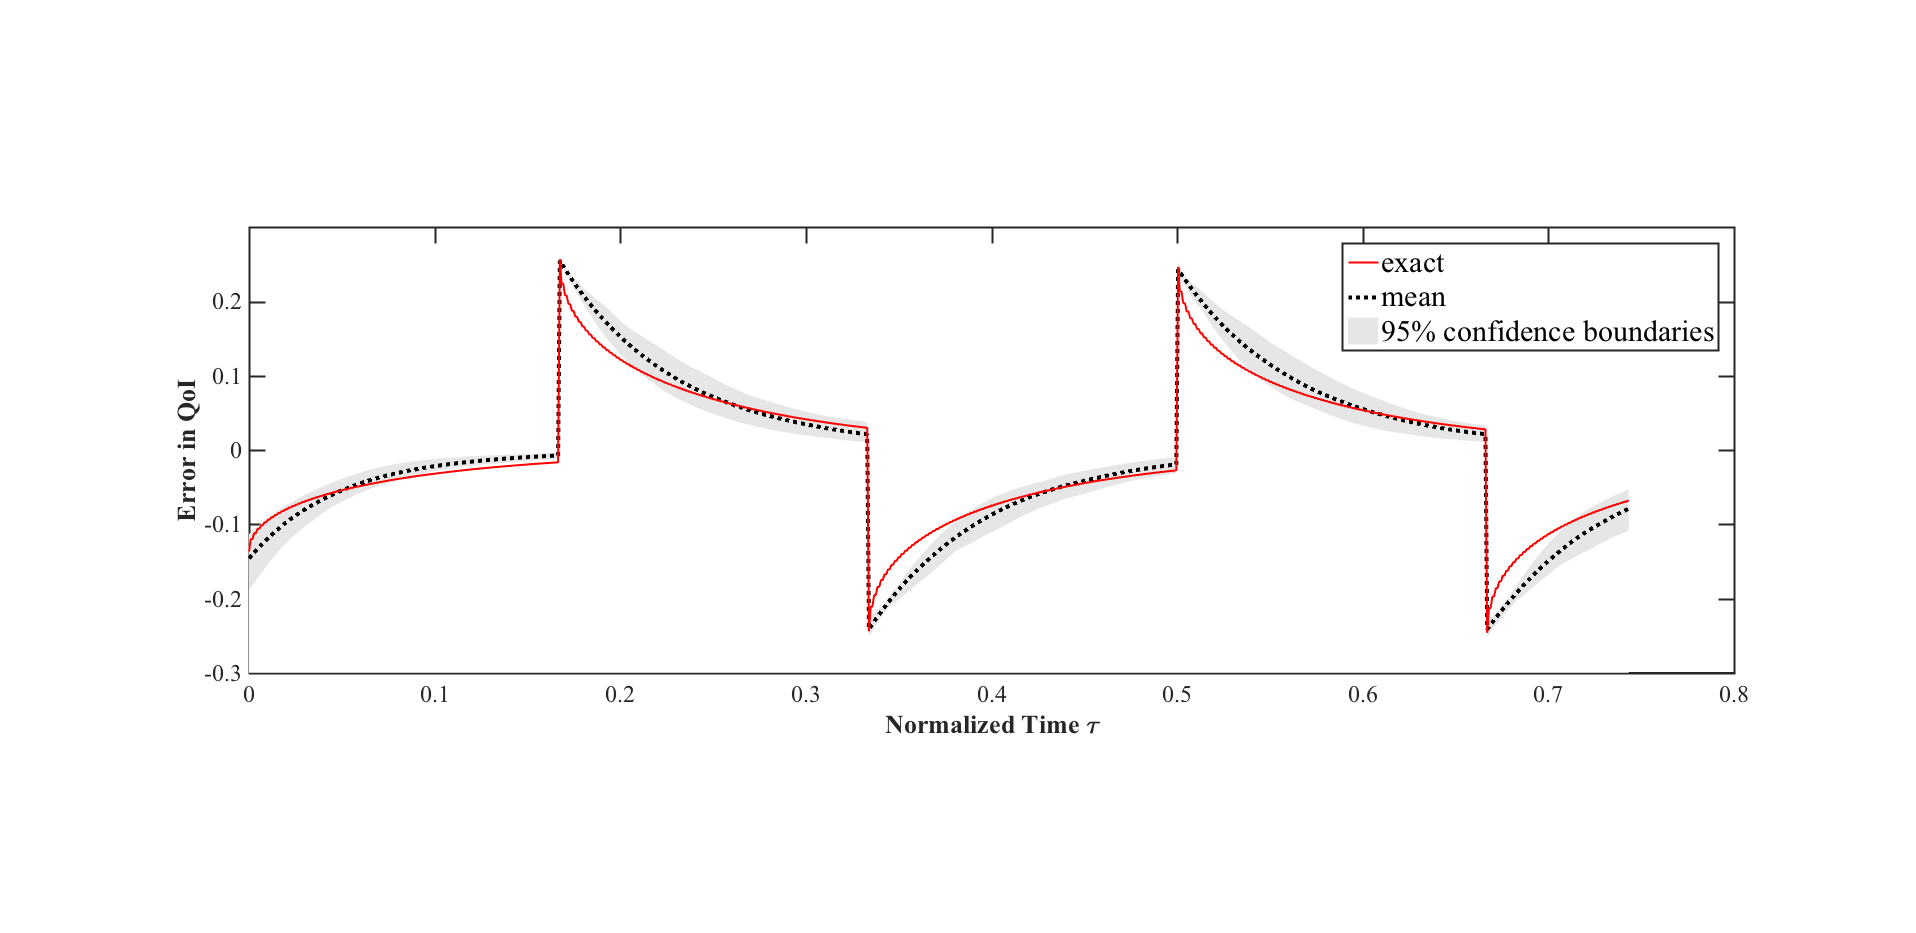
\includegraphics[trim = 1.3in 2.2in 1.6in 2.8in, clip, width=1\textwidth]{figs/error_bound.png} 
        \\
    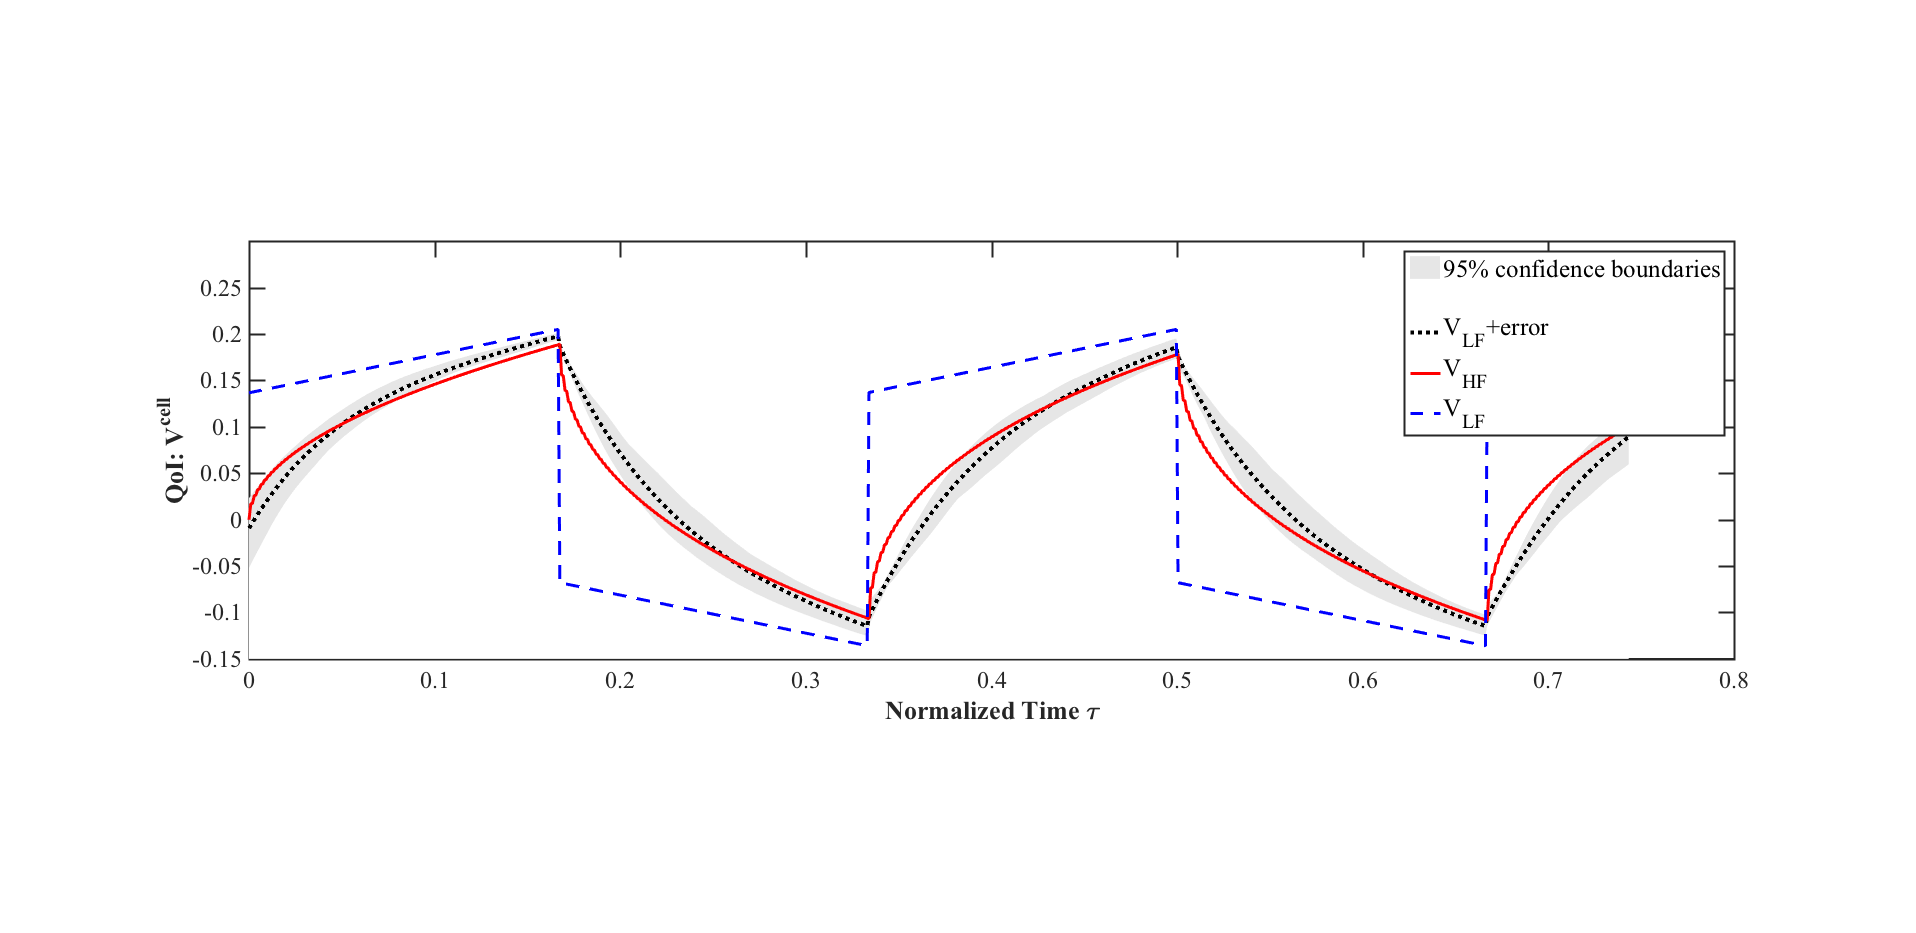
\includegraphics[trim = 1.3in 2.2in 1.6in 2.8in, clip, width=1\textwidth]{figs/V_bound.png} 
\end{figure}
\end{center}
\end{column}
\end{columns}
%====================
\begin{block}{}
\begin{itemize}
\item The ODE accounts for some of hidden features of HF i.e. 
the term $\lambda\epsilon$ takes care of the Kernel $\mathcal{K}$ and
the term $\alpha \frac{\partial I}{\partial\tau}$ accounts for discontinuity of $I$.
\item It needs to be trained by HF data i.e. calibrating parameters of inadequacy representation $(\alpha, \beta, c, \lambda_{mean})$. 
\end{itemize}
\end{block}


\vfill
\end{frame}


%===============================================================================
% Slide 03
%===============================================================================
\begin{frame}
\frametitle{Model Inadequacy - Version I}
\vfill


\begin{block}{Problems with deterministic part of the current ODE}
\begin{itemize}
\item It does not capture the short time behavior after sudden change in current.
\item It does not account for a wide range of current frequency. 
\end{itemize}
\end{block}

\begin{figure}[h]
    \centering
    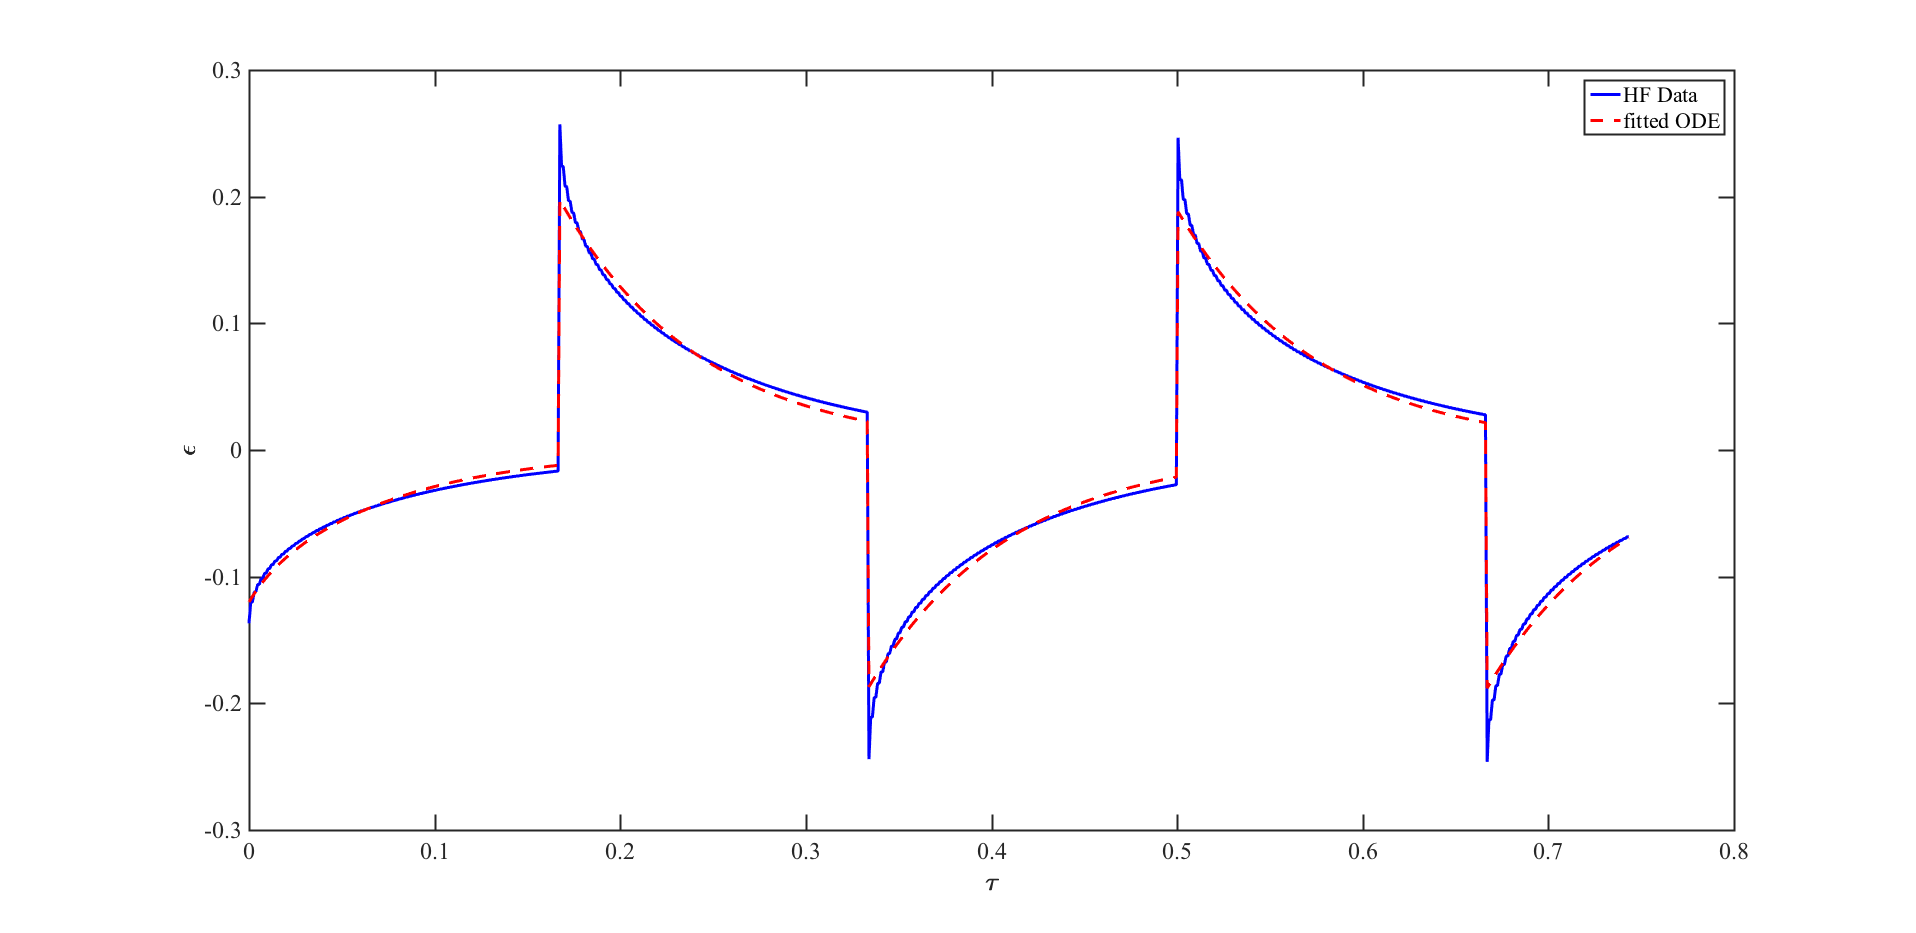
\includegraphics[trim = 1.6in 0.2in 1.6in 0.2in, clip, width=0.9\textwidth]{figs/step_optim_oldInad.png} 
    \vspace{-4mm}
\caption{Step change current.}
\end{figure}


\vfill
\end{frame}


%===============================================================================
% Slide 05
%===============================================================================
\begin{frame}
\frametitle{Model Inadequacy - Version I}
\vfill

\textbf{Sinusoidal current:}

\begin{figure}[h]
    \centering
    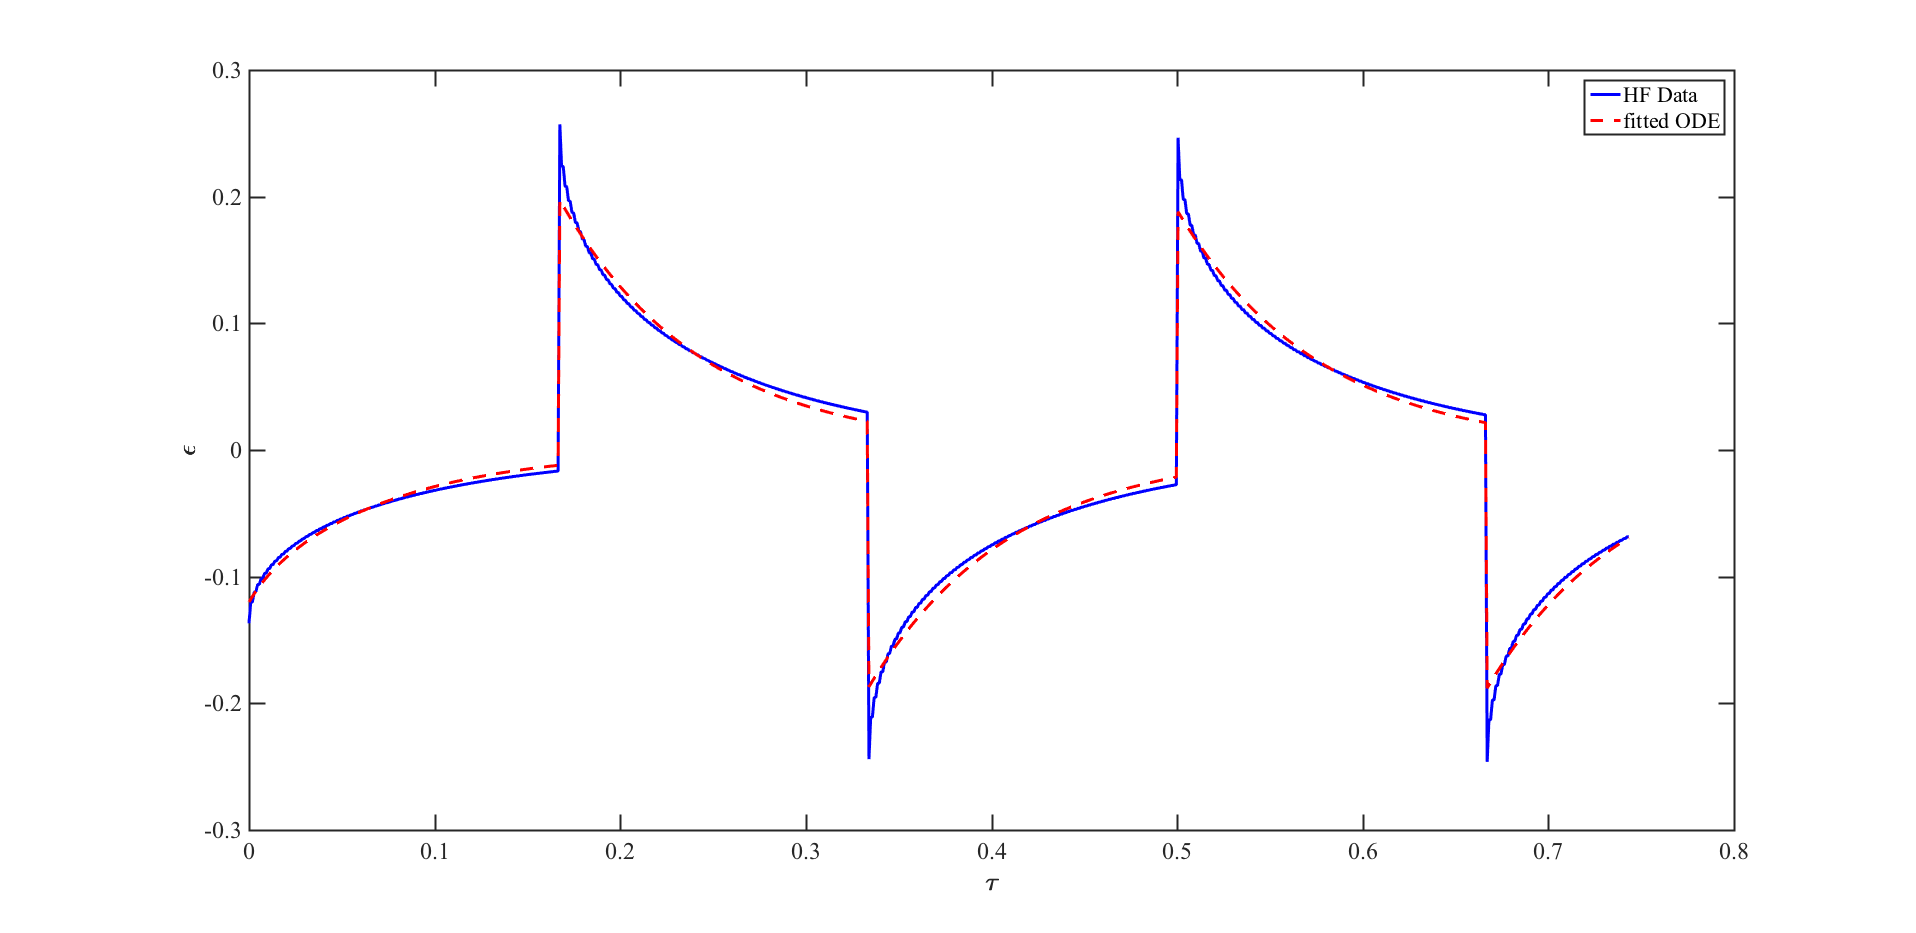
\includegraphics[trim = 1.6in 0.2in 1.6in 0.2in, clip, width=0.4\textwidth]{figs/step_optim_oldInad.png} 
    ~
    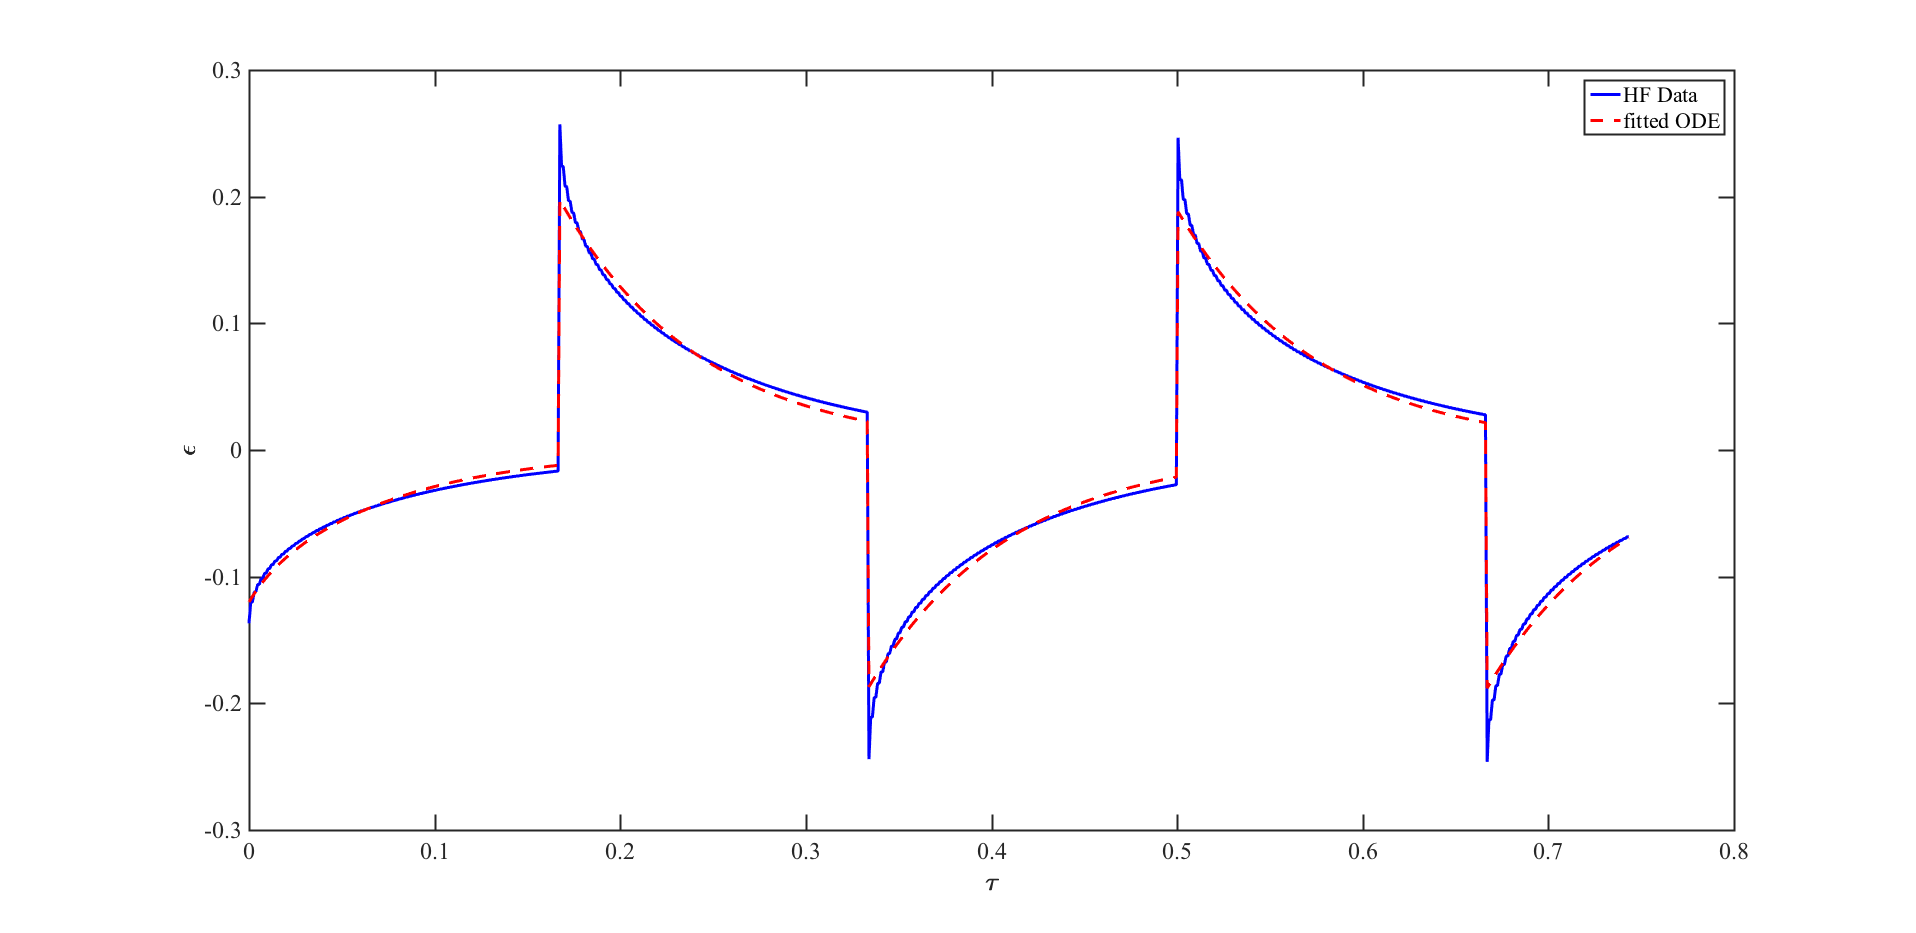
\includegraphics[trim = 1.6in 0.2in 1.6in 0.2in, clip, width=0.4\textwidth]{figs/step_optim_oldInad.png} 
    \vspace{-4mm}
\caption{(a) $I = \sin (50\tau)$. (b) $I = \sin (10\tau)$}
\end{figure}


\vfill
\end{frame}


%===============================================================================
% Slide 06
%===============================================================================
\begin{frame}
\frametitle{Model Inadequacy - Version I}
\vfill

\textbf{Sinusoidal current:}

\begin{figure}[h]
    \centering
    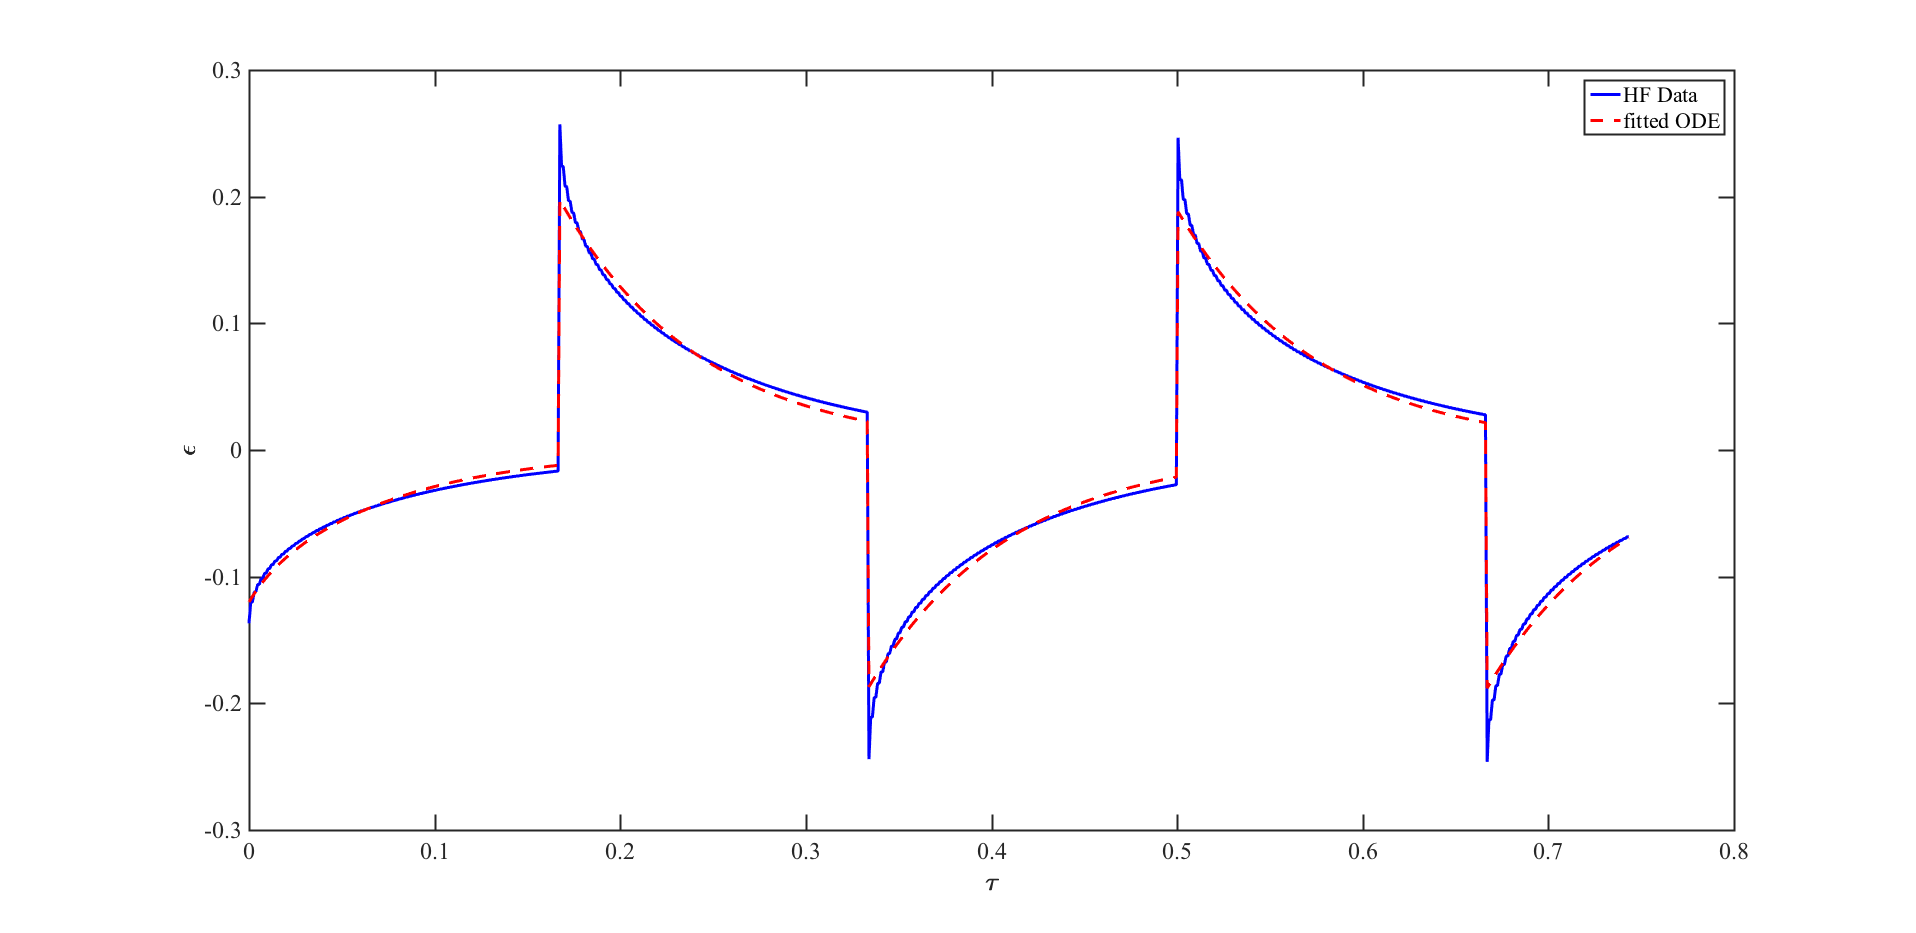
\includegraphics[trim = 1.6in 0.2in 1.6in 0.2in, clip, width=0.4\textwidth]{figs/step_optim_oldInad.png} 
    ~
    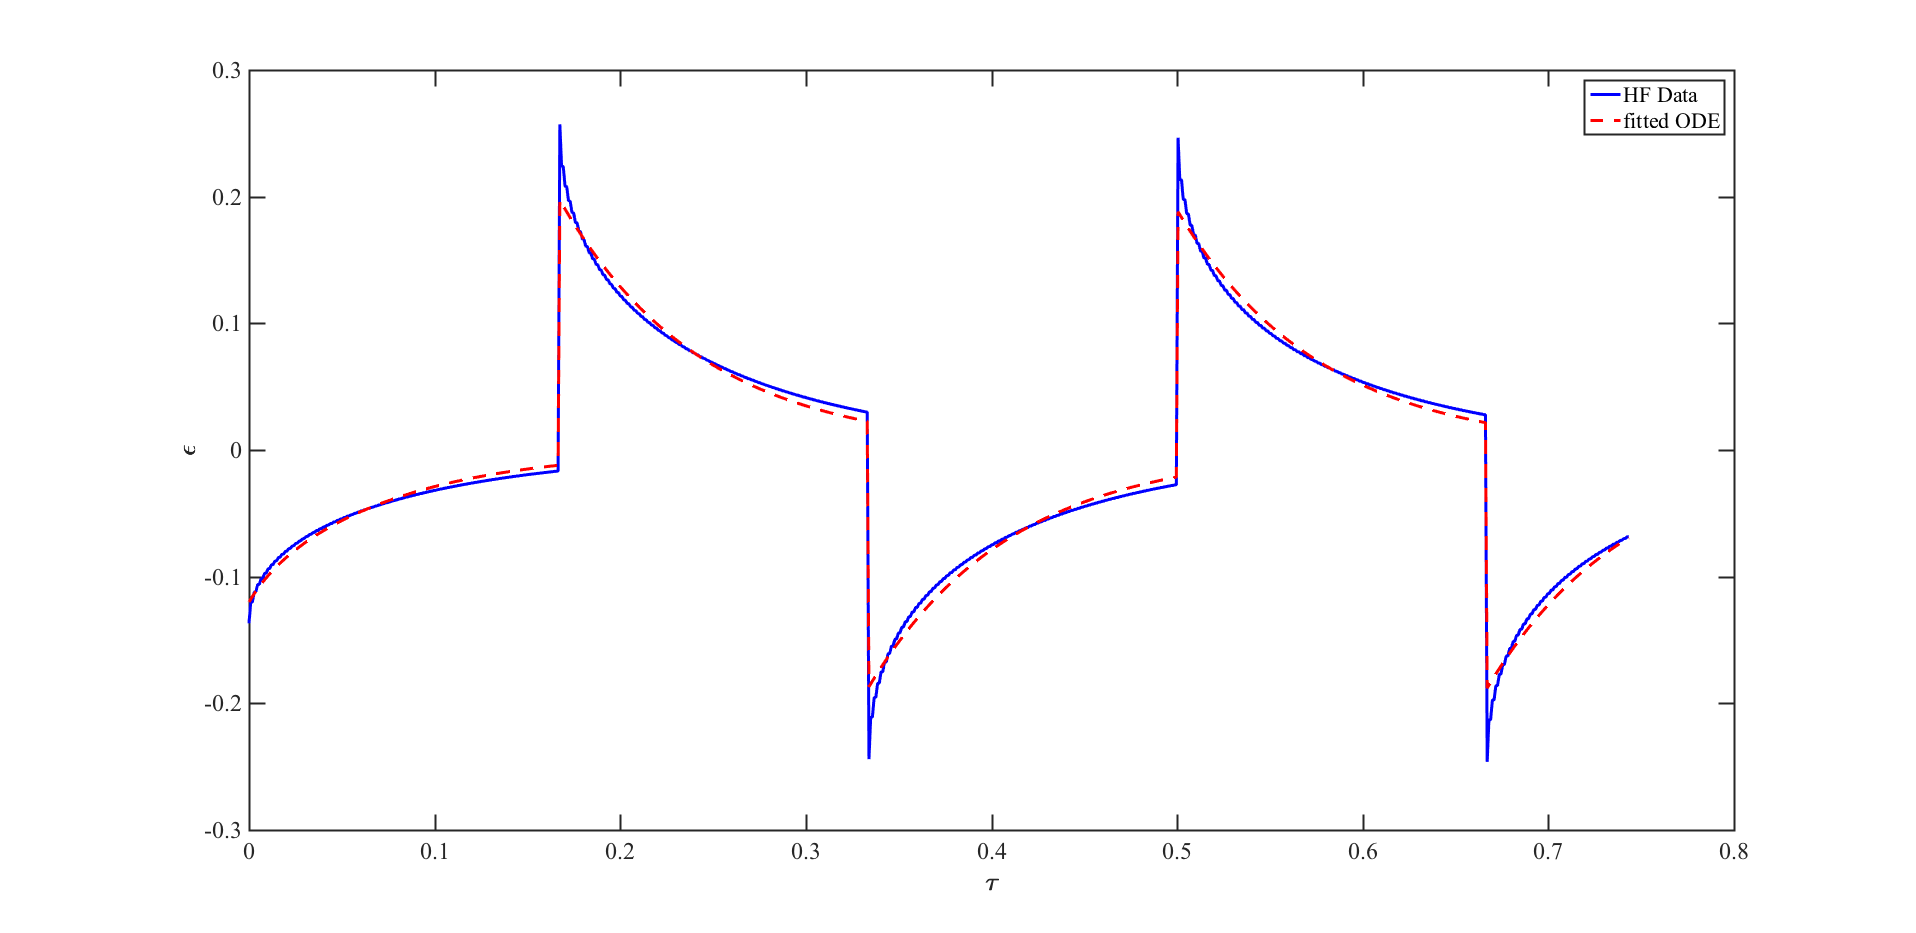
\includegraphics[trim = 1.6in 0.2in 1.6in 0.2in, clip, width=0.4\textwidth]{figs/step_optim_oldInad.png} 
    \vspace{-4mm}
\caption{(a) $I = \sin (50\tau)$. (b) $I = \sin (10\tau)$}
\end{figure}


\vfill
\end{frame}


%===============================================================================
% Slide 07
%===============================================================================
\begin{frame}
\frametitle{Closer look at behavior of over potential:}
\vfill


\begin{figure}[h]
    \centering
    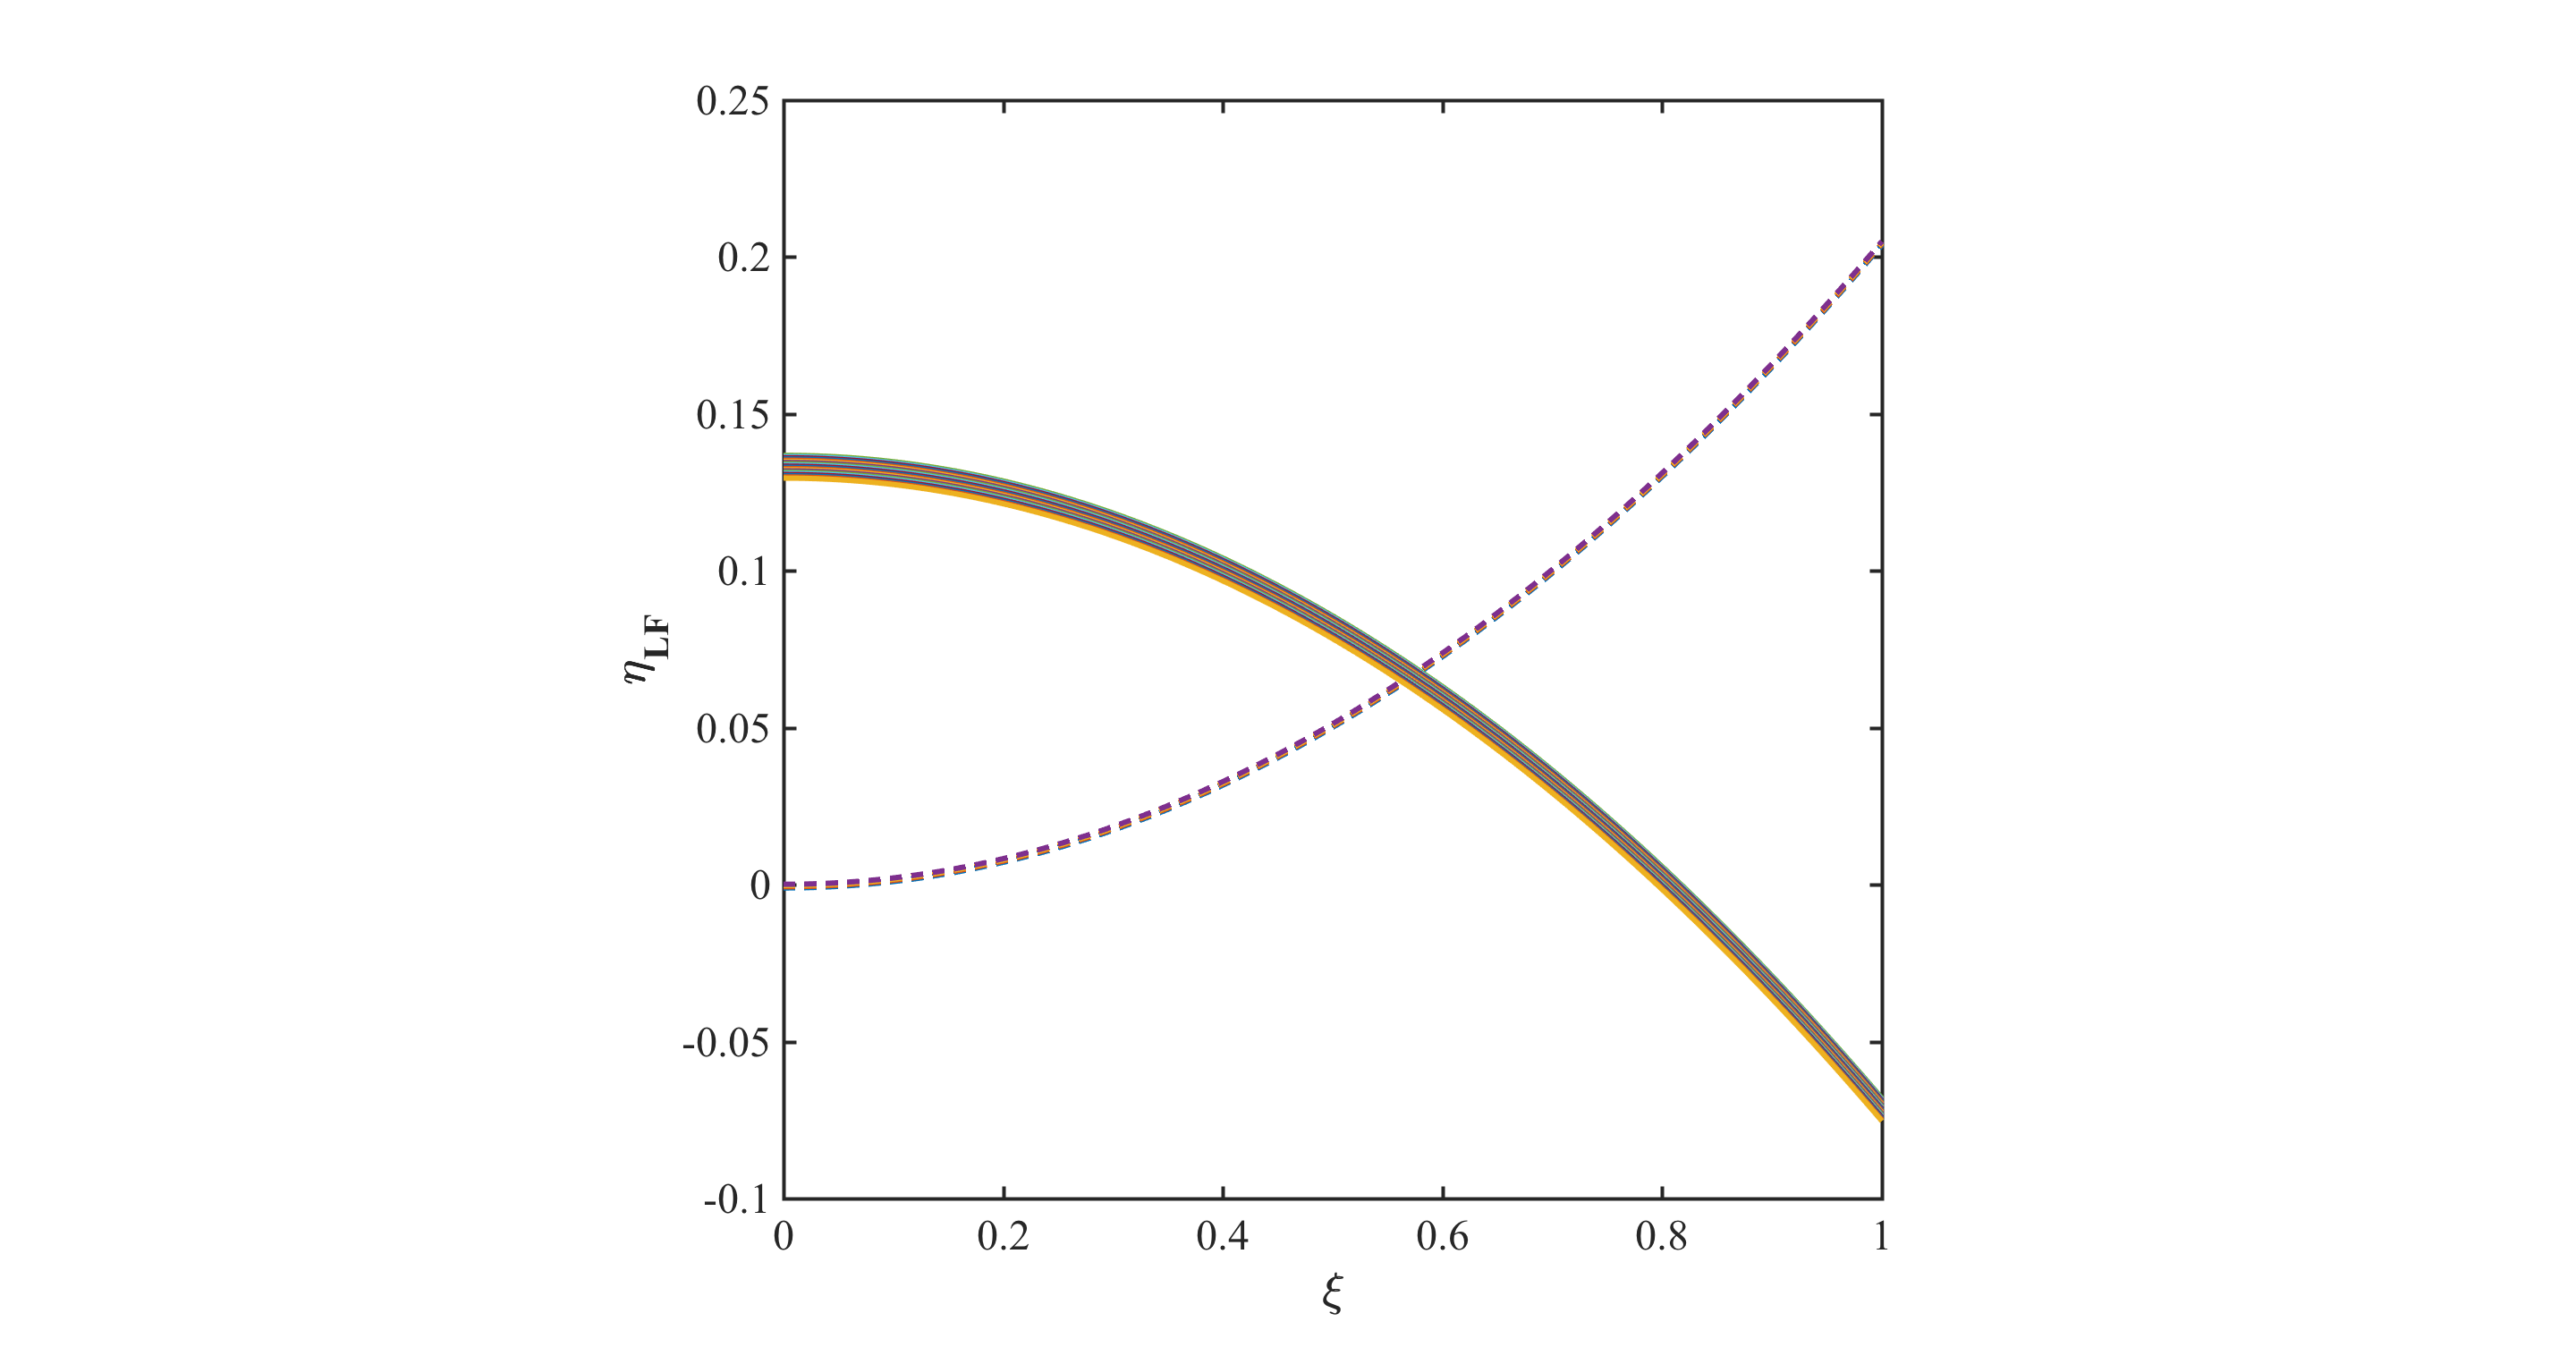
\includegraphics[trim = 9.6in 0.2in 9.6in 0.2in, clip, width=0.47\textwidth]{figs/eta_LF.png} 
    ~
    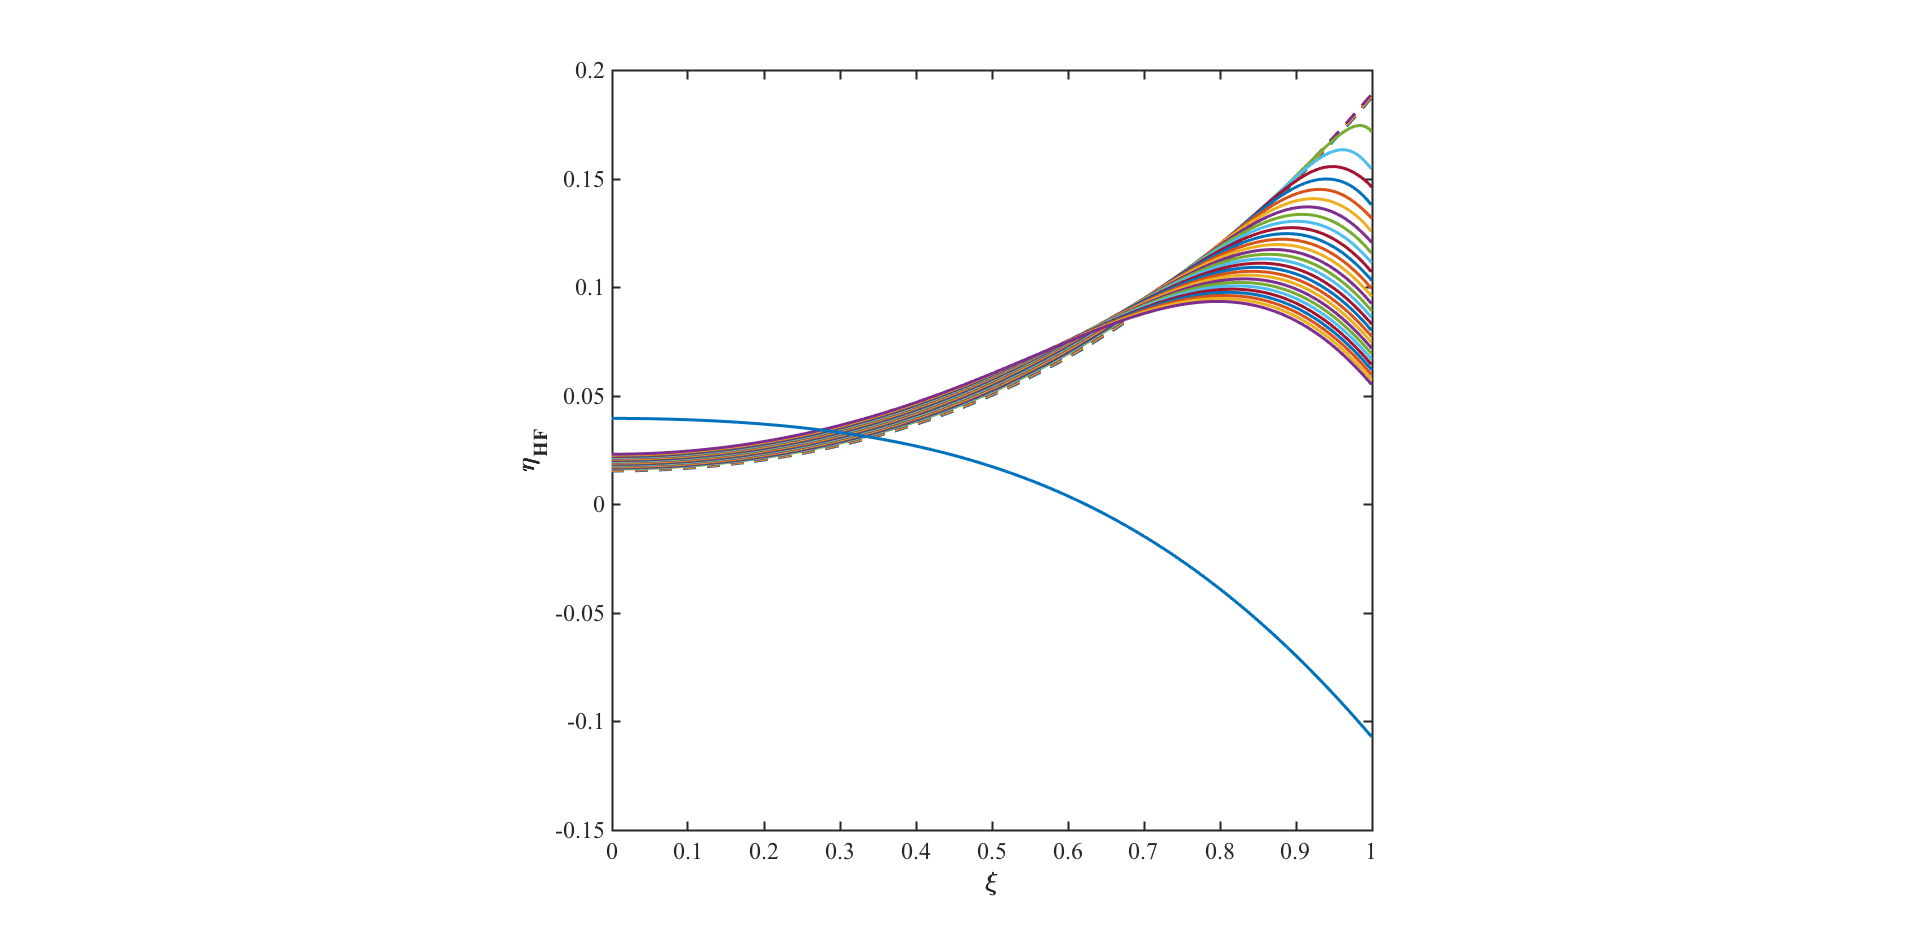
\includegraphics[trim = 7in 0.2in 7in 0.2in, clip, width=0.47\textwidth]{figs/eta_HF.png}
        \vspace{-3mm}
\caption{Step change current when sign of current changes.} 
\end{figure}


\vfill
\end{frame}


%===============================================================================
% Slide 08
%===============================================================================
\begin{frame}
\frametitle{Closer look at behavior of over potential:}
\vfill

\begin{center}
\textbf{\large Stokes's first problem with Neumann boundary condition}\\
on the board ...
\end{center}

\vfill
\end{frame}


%===============================================================================
% Slide 09
%===============================================================================
\begin{frame}
\frametitle{Model Inadequacy - Version II}
\vfill

\begin{itemize}
\item when current step changes, at the boundary and short time $\eta_{HF} \propto \sqrt{\tau}$.
\item since $\eta_{LF}$ changes rapidly at the boundary, one can conclude $\epsilon \propto \sqrt{\tau}$
\item from $\epsilon \propto \sqrt{\tau}$ one can infere $\frac{d\epsilon}{d\tau} \propto \frac{1}{\sqrt{\tau}}$
\end{itemize}

From above consideration, we postulated a possible inadequacy representation for short time after step change  as: 
\begin{equation*}
\frac{\partial\epsilon}{\partial\tau} = -\frac{\lambda}{\sqrt{\tau - {T}(\tau)}} + \alpha \frac{\partial I}{\partial\tau},
\end{equation*}
where ${T}(\tau) = \tau_{jump}$ in case of step change current. \textbf{plot on the board}

\begin{center}
Does this form works for long time also?
\end{center}

\vfill
\end{frame}


%===============================================================================
% Slide 10
%===============================================================================
\begin{frame}
\frametitle{Model Inadequacy - Version II}
\vfill

\textbf{Test Problem:}

\begin{eqnarray*}
{\rm option 1:} & \frac{\partial\epsilon}{\partial\tau} = -\frac{\lambda}{\sqrt{\tau - {T}(\tau)}} + \alpha \frac{\partial I}{\partial\tau}\\
{\rm option 2:} & \frac{\partial\epsilon}{\partial\tau} = -\frac{\lambda\epsilon}{\sqrt{\tau - {T}(\tau)}} + \alpha \frac{\partial I}{\partial\tau}
\end{eqnarray*}

\begin{figure}[h]
    \centering
    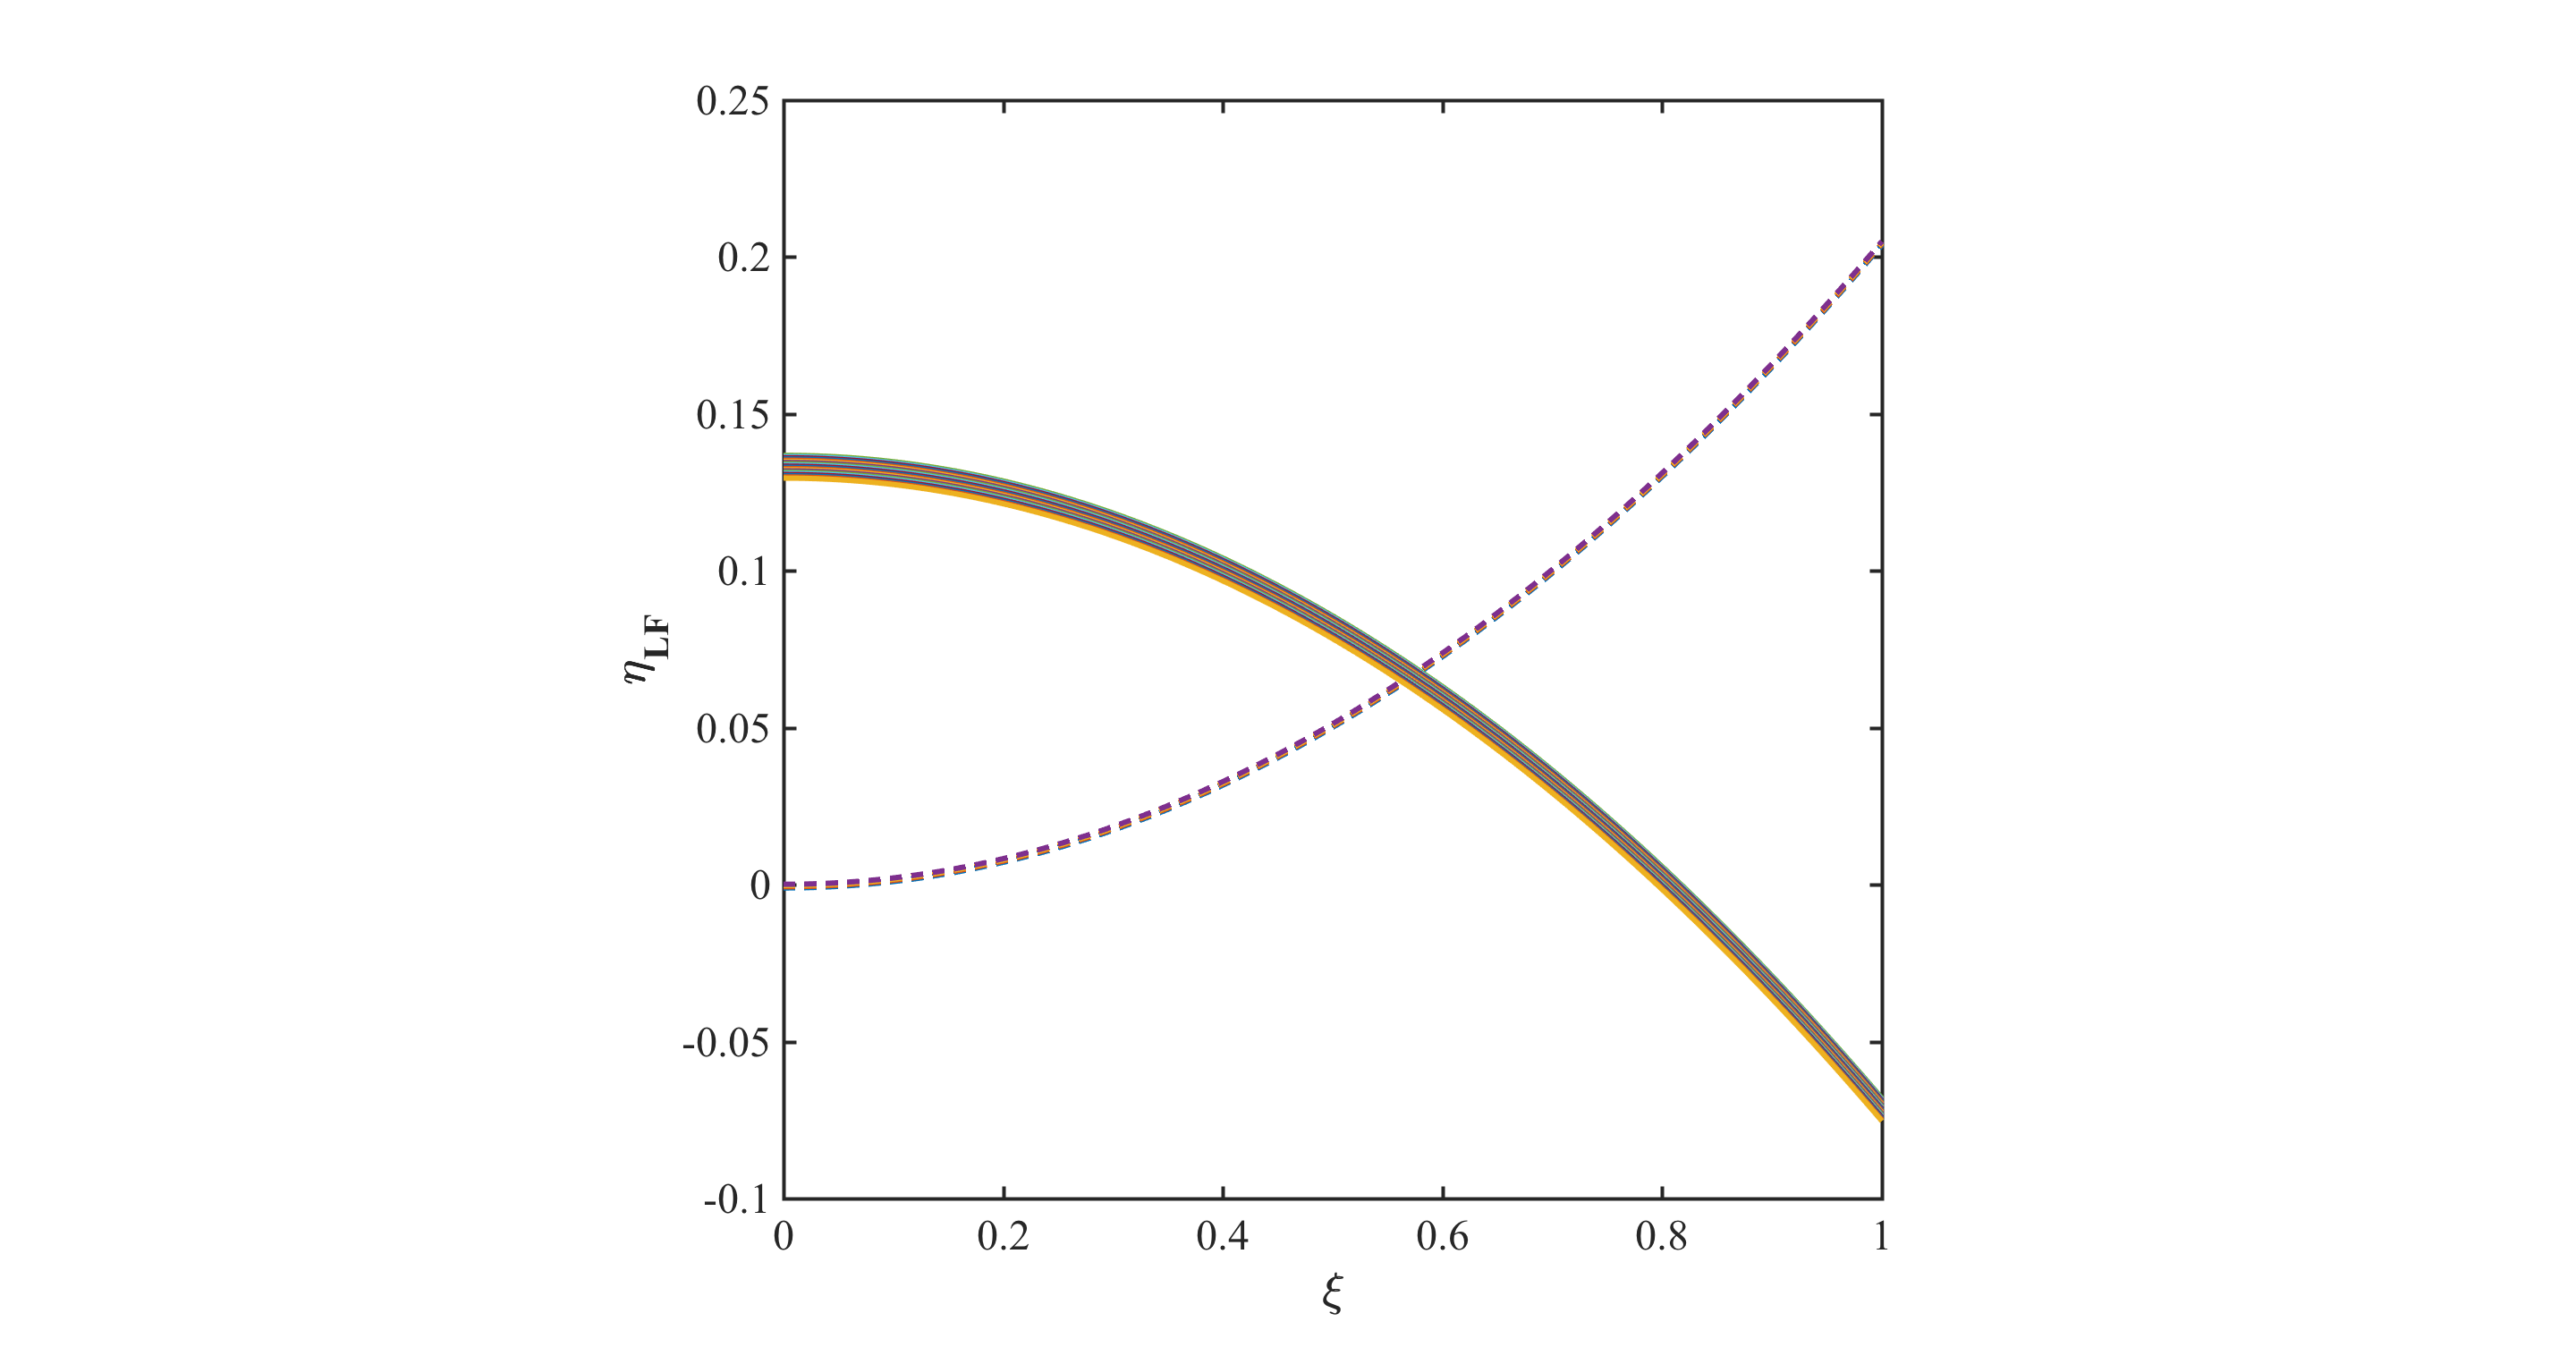
\includegraphics[trim = 9.6in 0.2in 9.6in 0.2in, clip, width=0.4\textwidth]{figs/eta_LF.png} 
    ~
    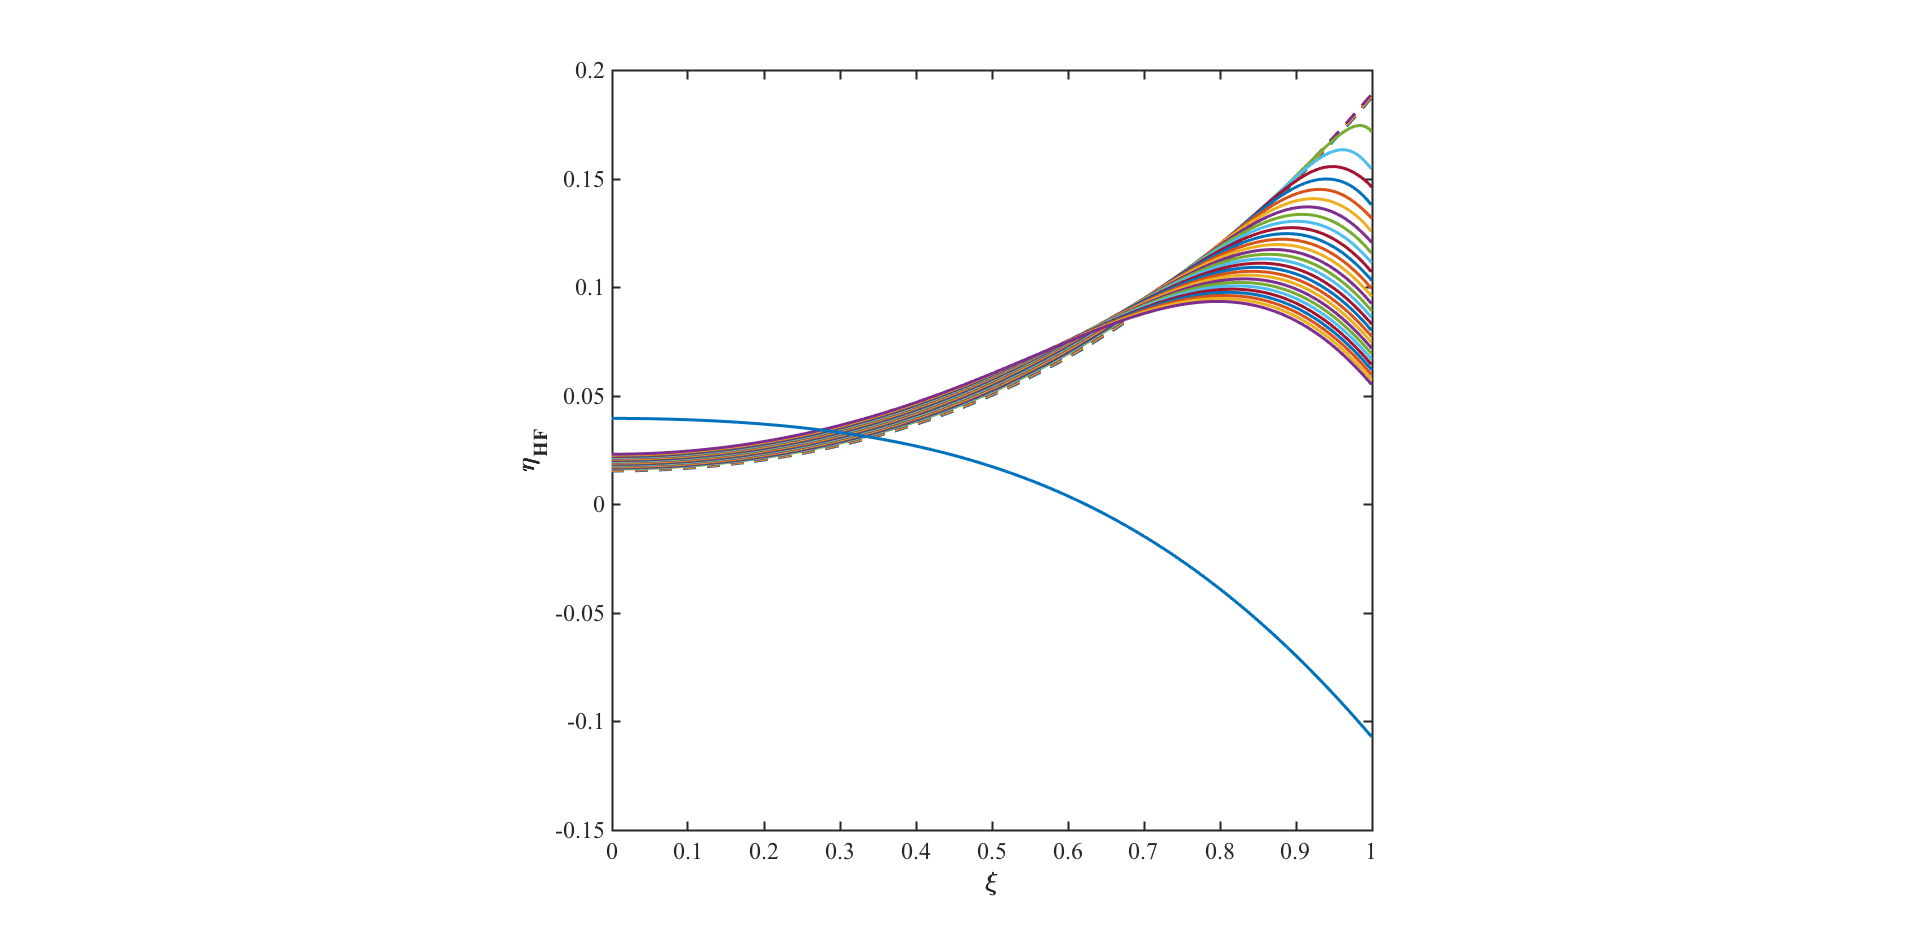
\includegraphics[trim = 7in 0.2in 7in 0.2in, clip, width=0.4\textwidth]{figs/eta_HF.png}
        \vspace{-3mm}
\caption{(a) change in current with time; (b) two inadequacy options calibrated with HF data.} 
\end{figure}


\vfill
\end{frame}


%===============================================================================
% Slide 11
%===============================================================================
\begin{frame}
\frametitle{Model Inadequacy - Version II}
\vfill


\begin{alertblock}{Inadequacy representation (v.2)}
\textbf{Auxiliary Stochastic ODE:}
\begin{equation*}
\frac{\partial\epsilon}{\partial\tau} = -\frac{\lambda\epsilon}{\sqrt{\tau - {T}(\tau)}} + \alpha \frac{\partial I}{\partial\tau}
\end{equation*}

where $\lambda$ and $\alpha$ are parameters of inadequacy representation. 
\end{alertblock}



\textbf{What is a general form for $T(\tau) \propto I(\tau)$?}

\begin{itemize}
\item $T(\tau)$ should be consistent with what we expect in step changes current.
\item In sinusoidal current it seems $T(\tau)$ should take care of lagging time between HF and LF model.
\end{itemize}


From above consideration, we postulated a possible evolution equation for ${T}(\tau)$ as: 
\begin{equation*}
\frac{\partial T}{\partial\tau} = (\tau - T(\tau)) \left| \frac{\partial I}{\partial\tau} \right|
\end{equation*}


\vfill
\end{frame}

















\end{document}
